\chapter{KIỂM ĐỊNH TÍNH NGẪU NHIÊN}
\section{Thiết kế giả thuyết và hiệu chỉnh đa kiểm định}
Phần P1 kiểm tra liệu dữ liệu có lệch khỏi các mô hình ngẫu nhiên cơ bản hay không. Mỗi nhóm kiểm định được thực hiện trên dữ liệu gộp và/hoặc theo vị trí chữ số, sau đó p-value được hiệu chỉnh bằng thủ tục Benjamini--Hochberg với ngưỡng $q<0{,}05$. Cách làm này hạn chế kết luận sai do số lượng kiểm định lớn.

\begin{table}[H]\centering
\caption{Số kiểm định và kết quả sau hiệu chỉnh FDR}
\begin{tabular}{lrr}\toprule
Nhóm kiểm định & Số kiểm định & Bác bỏ $H_0$\\\midrule
Phân phối chữ số & 45 & 1\\
Phân phối đuôi số & 28 hợp lệ & 5\\
Độc lập giữa vị trí & 90 & 0\\
Markov lag 1 & 90 & 0\\
Phụ thuộc lag 1--30 & 2700 & 0\\
Ổn định theo giai đoạn & 4050 & 0\\\bottomrule
\end{tabular}\end{table}

\section{Phân phối chữ số và phân phối đuôi số}
Kiểm định $\chi^2$ được dùng để so sánh tần suất chữ số quan sát với phân phối đều. Hình~\ref{fig:p1-digit} cho thấy các sai khác biên trong dữ liệu gộp; chỉ một trong 45 kiểm định còn ý nghĩa sau FDR. Với các đuôi số, chỉ 28 kiểm định đủ điều kiện và có 5 bác bỏ $H_0$. Đây là các phát hiện cục bộ, chưa đủ để kết luận tồn tại quy luật tổng quát.
\begin{figure}[H]\centering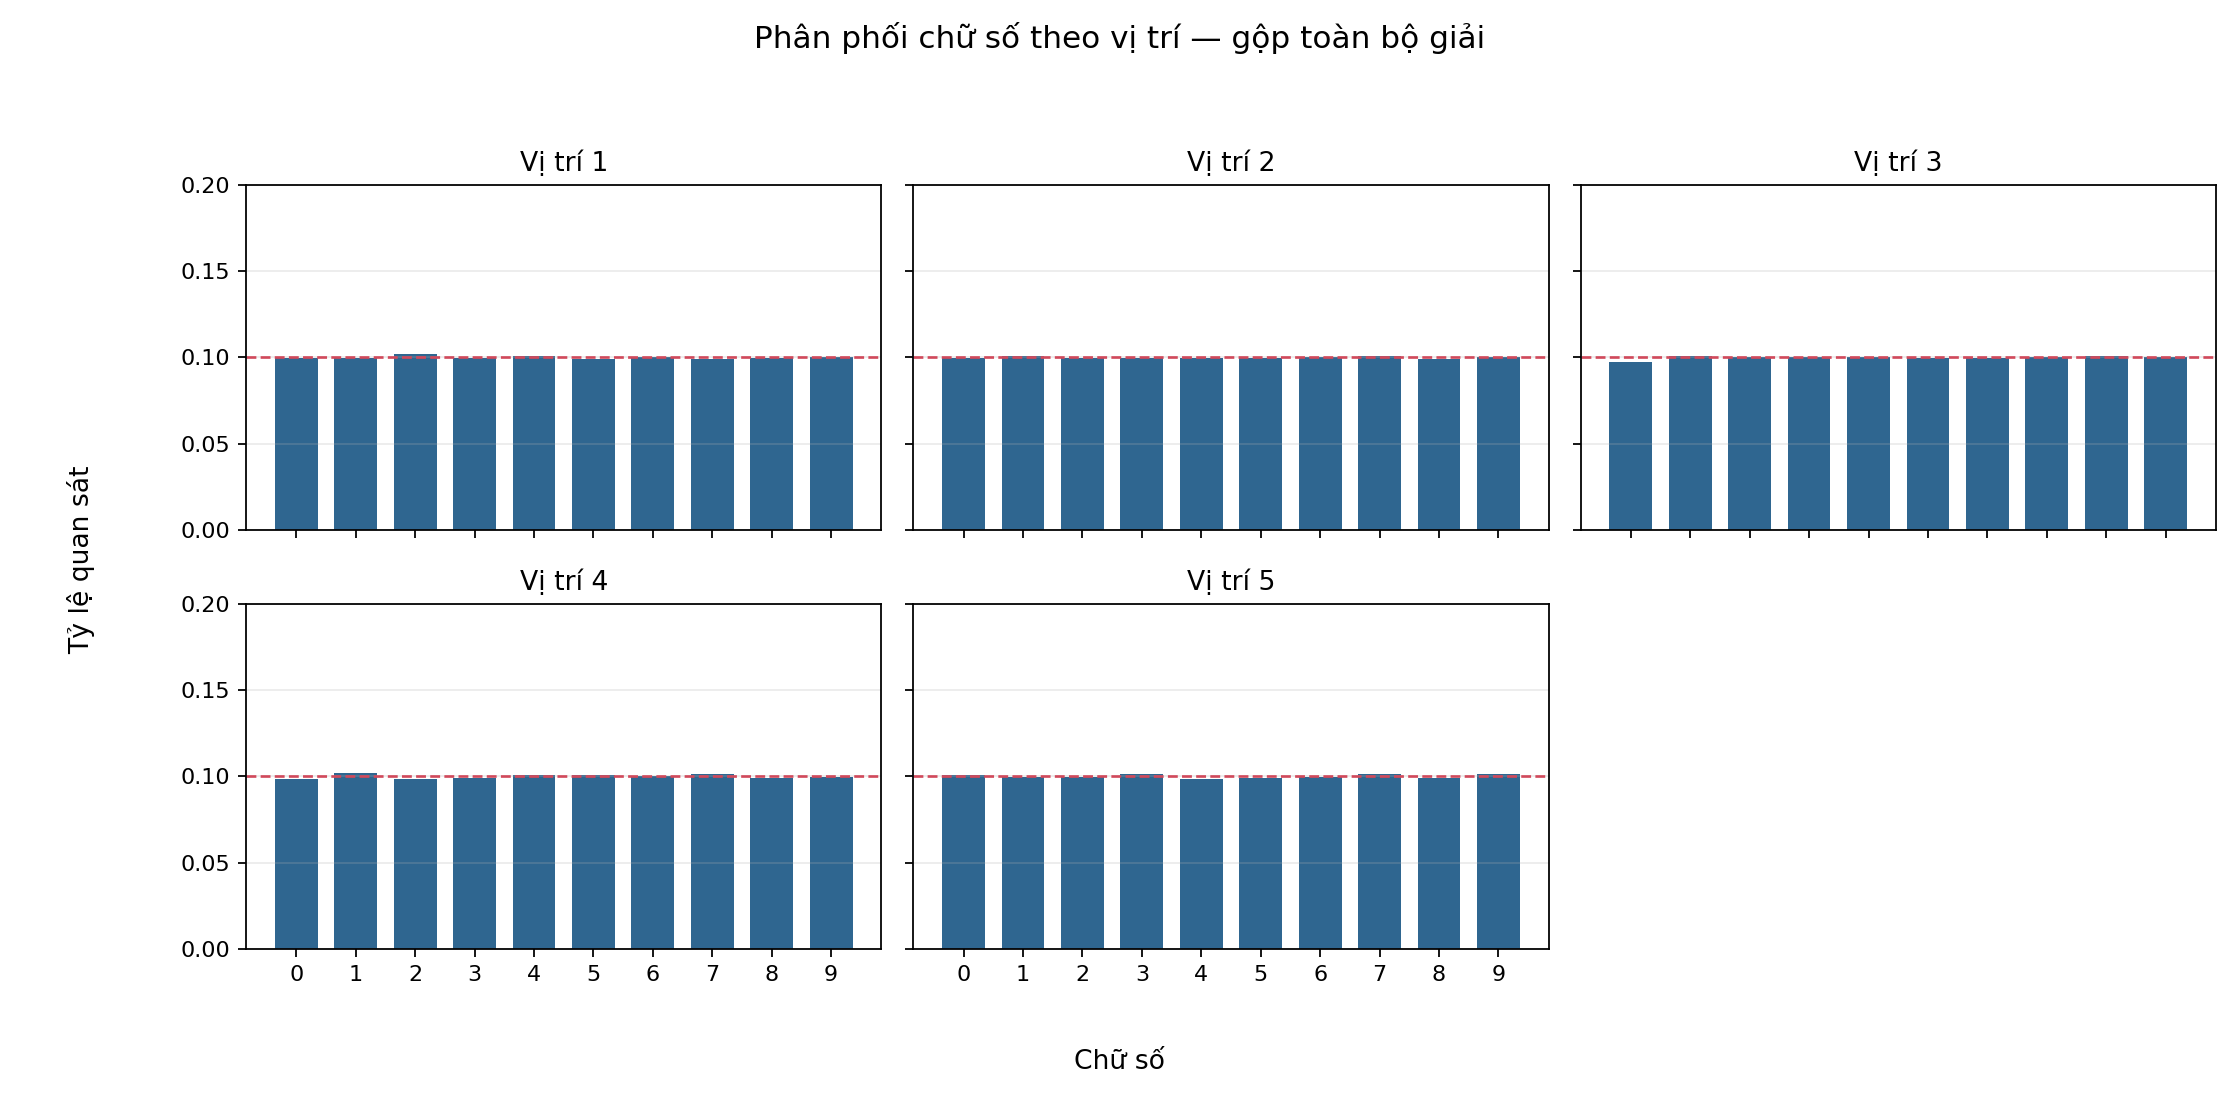
\includegraphics[width=0.92\linewidth]{../artifacts/p1_statistical_tests/01_digit_distribution/figures/01_pooled_digit_distribution.png}\caption{Phân phối chữ số theo vị trí trong toàn bộ dữ liệu.}\label{fig:p1-digit}\end{figure}

\section{Độc lập giữa các vị trí}
Kiểm định độc lập và thống kê liên hợp được dùng để xem chữ số ở các vị trí có liên hệ vượt quá mức kỳ vọng hay không. Không có bác bỏ nào trong 90 kiểm định sau FDR. Hình~\ref{fig:p1-position} trực quan hóa mức phụ thuộc rất nhỏ giữa các vị trí.
\begin{figure}[H]\centering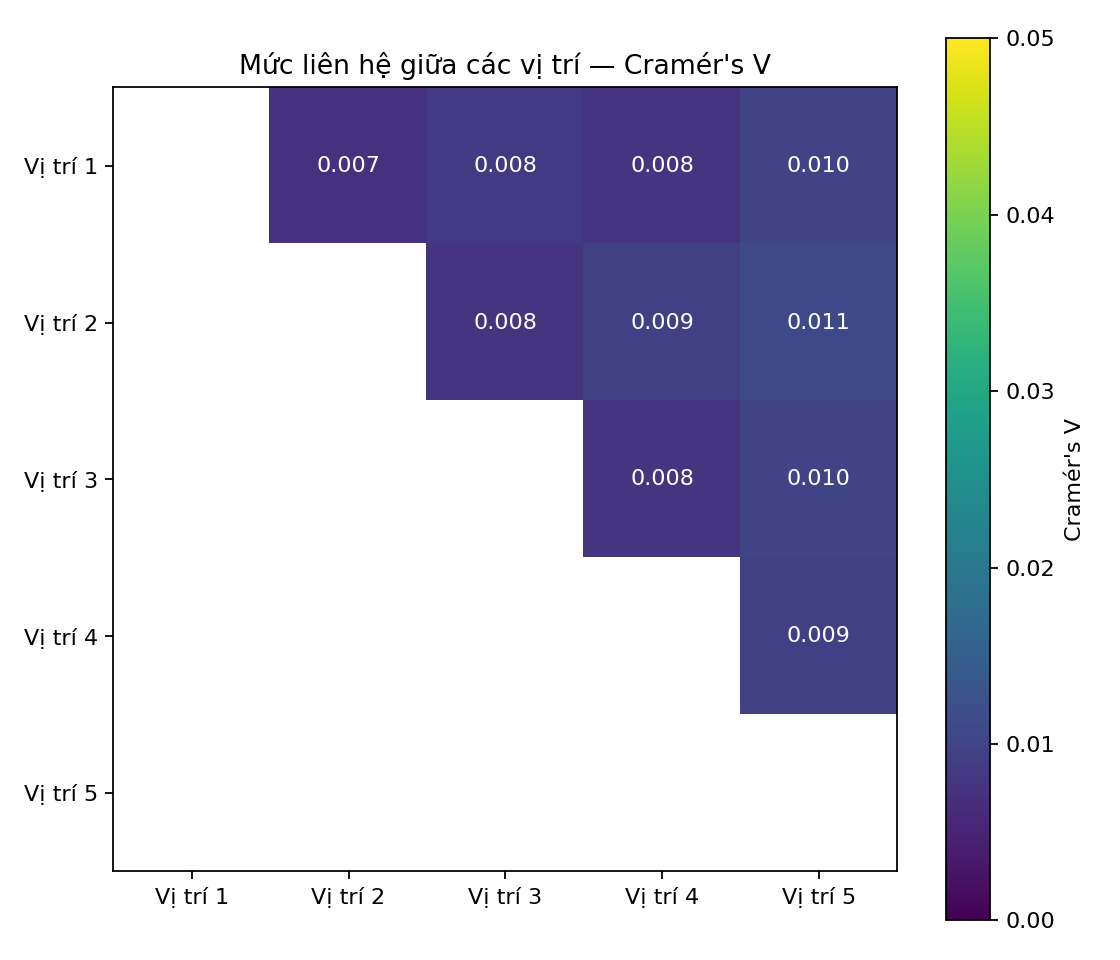
\includegraphics[width=0.92\linewidth]{../artifacts/p1_statistical_tests/02_position_independence/figures/02_pooled_position_dependence.png}\caption{Mức phụ thuộc giữa các vị trí chữ số.}\label{fig:p1-position}\end{figure}

\section{Phụ thuộc Markov và phụ thuộc theo độ trễ}
P1 kiểm tra cả phụ thuộc chuyển trạng thái ở lag 1 và phụ thuộc giữa các ngày ở lag 1--30. Không có kiểm định Markov nào trong 90 kiểm định bị bác bỏ; hình~\ref{fig:p1-markov} cho thấy độ lệch chuyển trạng thái không tạo cấu trúc nổi bật. Tương tự, thống kê Cramér's V theo các độ trễ không cho thấy tín hiệu bền vững (Hình~\ref{fig:p1-lag}).
\begin{figure}[H]\centering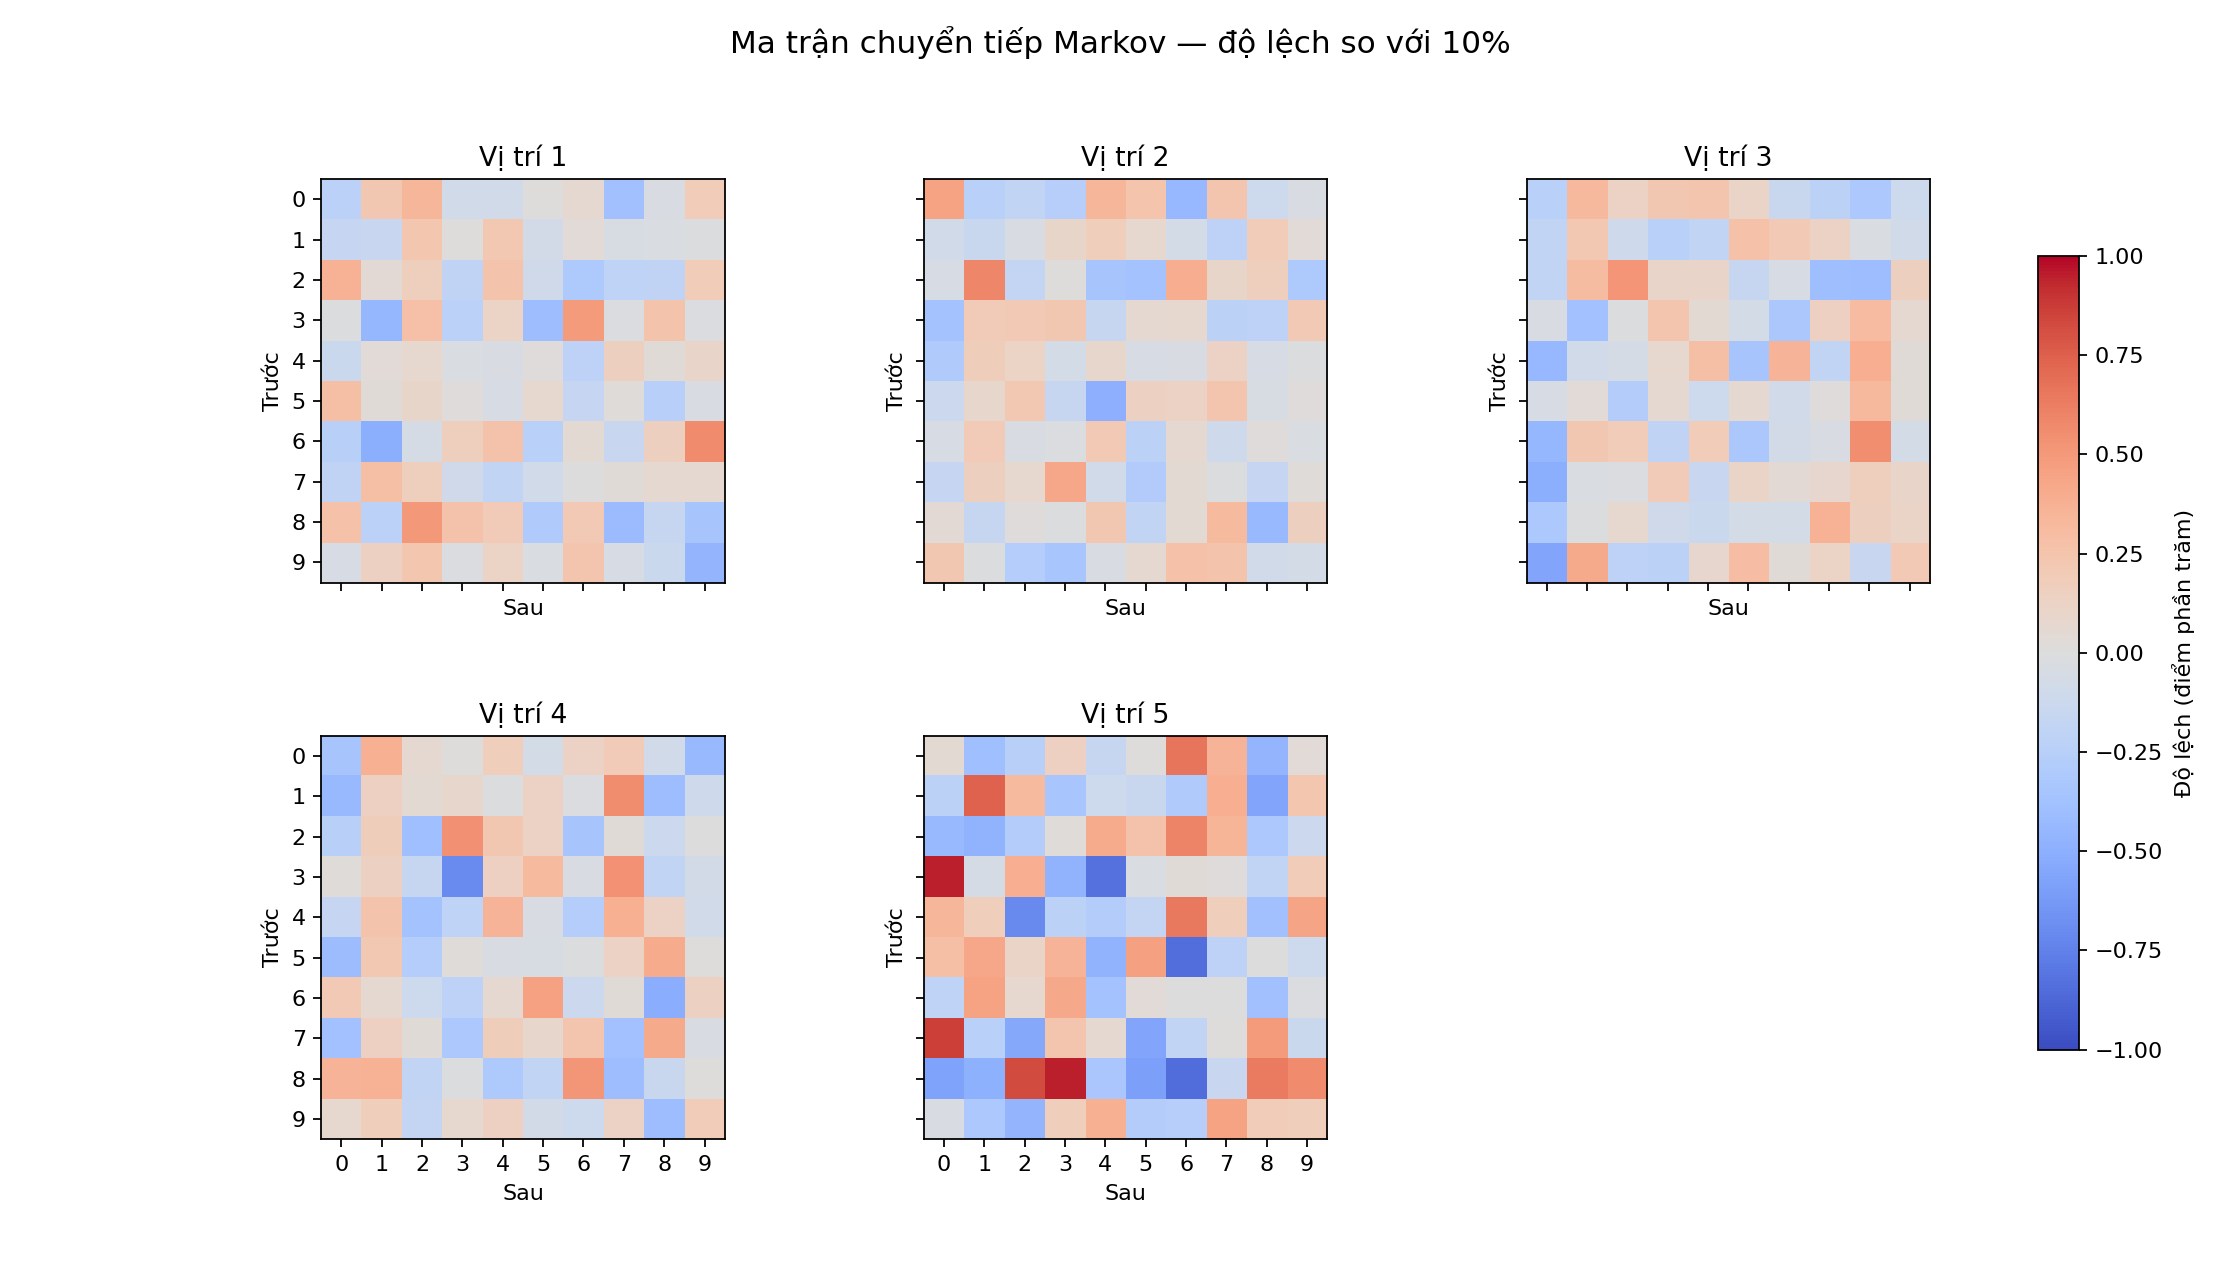
\includegraphics[width=0.92\linewidth]{../artifacts/p1_statistical_tests/03_markov_by_position/figures/01_transition_deviations.png}\caption{Độ lệch của ma trận chuyển trạng thái Markov lag 1.}\label{fig:p1-markov}\end{figure}
\begin{figure}[H]\centering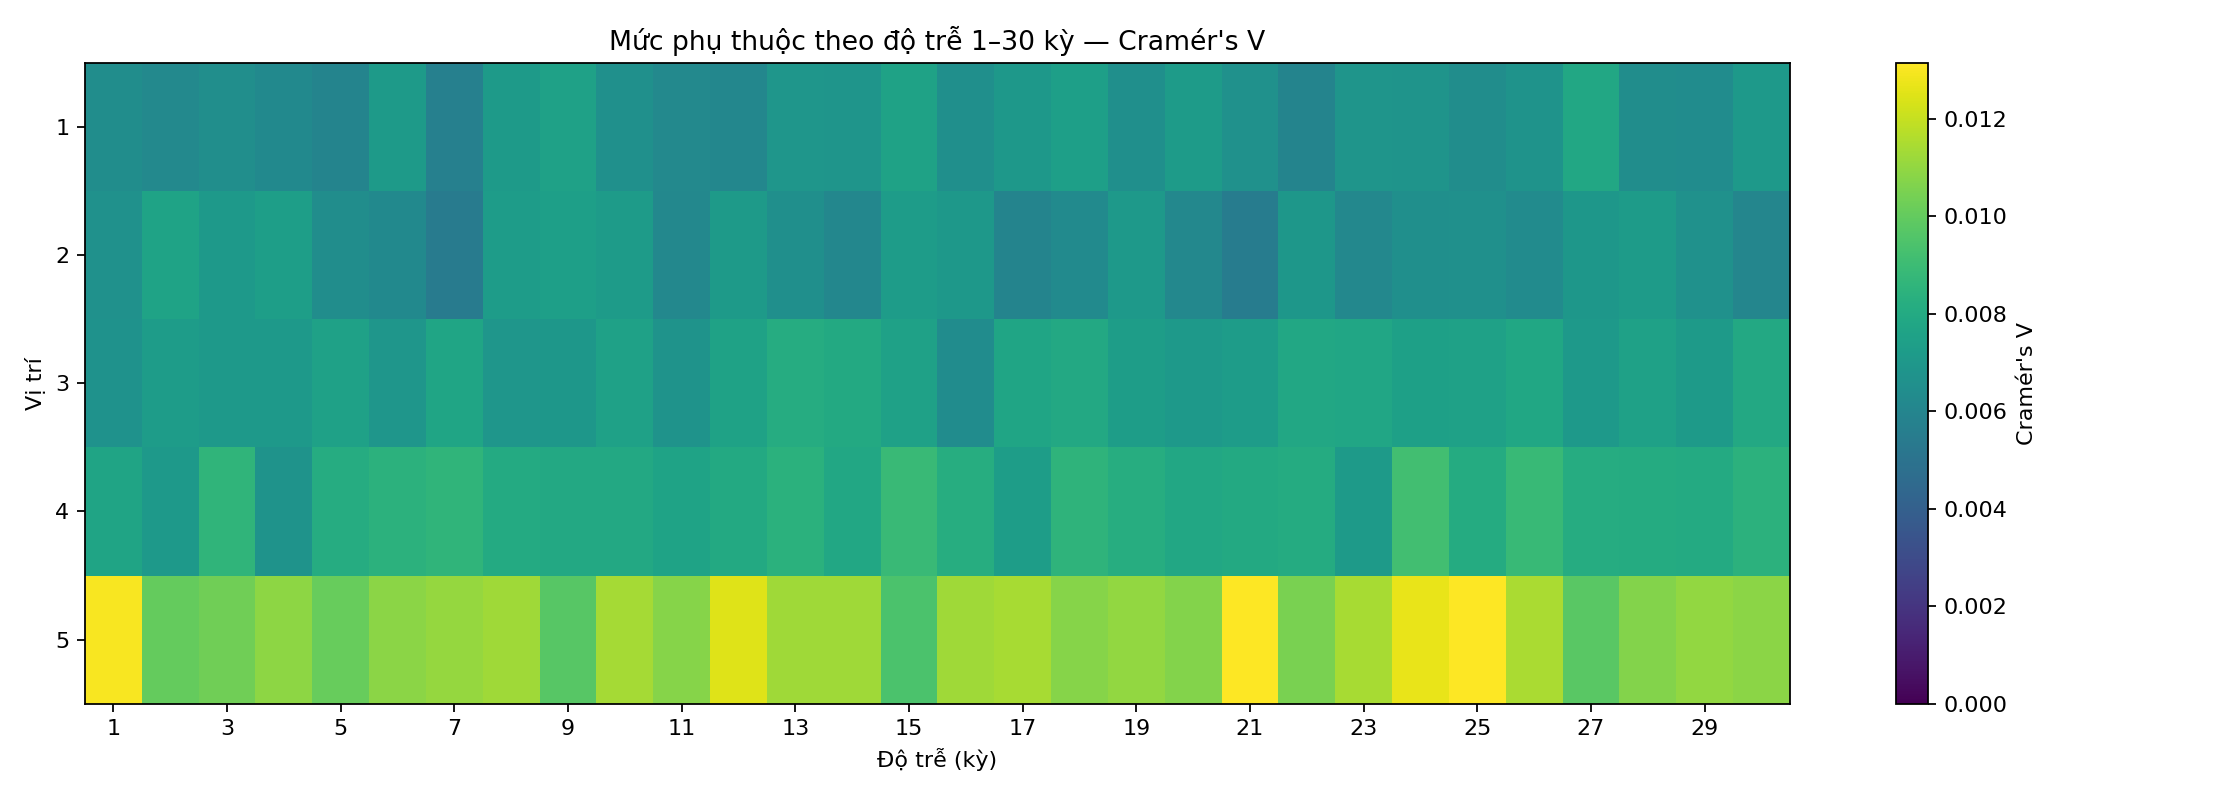
\includegraphics[width=0.92\linewidth]{../artifacts/p1_statistical_tests/04_temporal_randomness/figures/04_lag_dependence_cramers_v.png}\caption{Phụ thuộc theo độ trễ 1--30 ngày bằng Cramér's V.}\label{fig:p1-lag}\end{figure}

\section{Ổn định theo thời gian và trúng đồng thời}
Phân tích ổn định chia chuỗi theo giai đoạn và lặp lại các kiểm định chính. Không có bác bỏ nào trong 4050 kiểm định; Hình~\ref{fig:p1-stability} tóm tắt kết quả ý nghĩa theo từng nhóm. Tỷ lệ ngày có ít nhất hai giải cùng chứa một đuôi số là 62,63\%; ít nhất ba giải là 0,25\%; ít nhất bốn giải xấp xỉ 0,00\%. Đây là mô tả cơ chế chồng lấn của nhiều giải, không phải bằng chứng dự báo.
\begin{figure}[H]\centering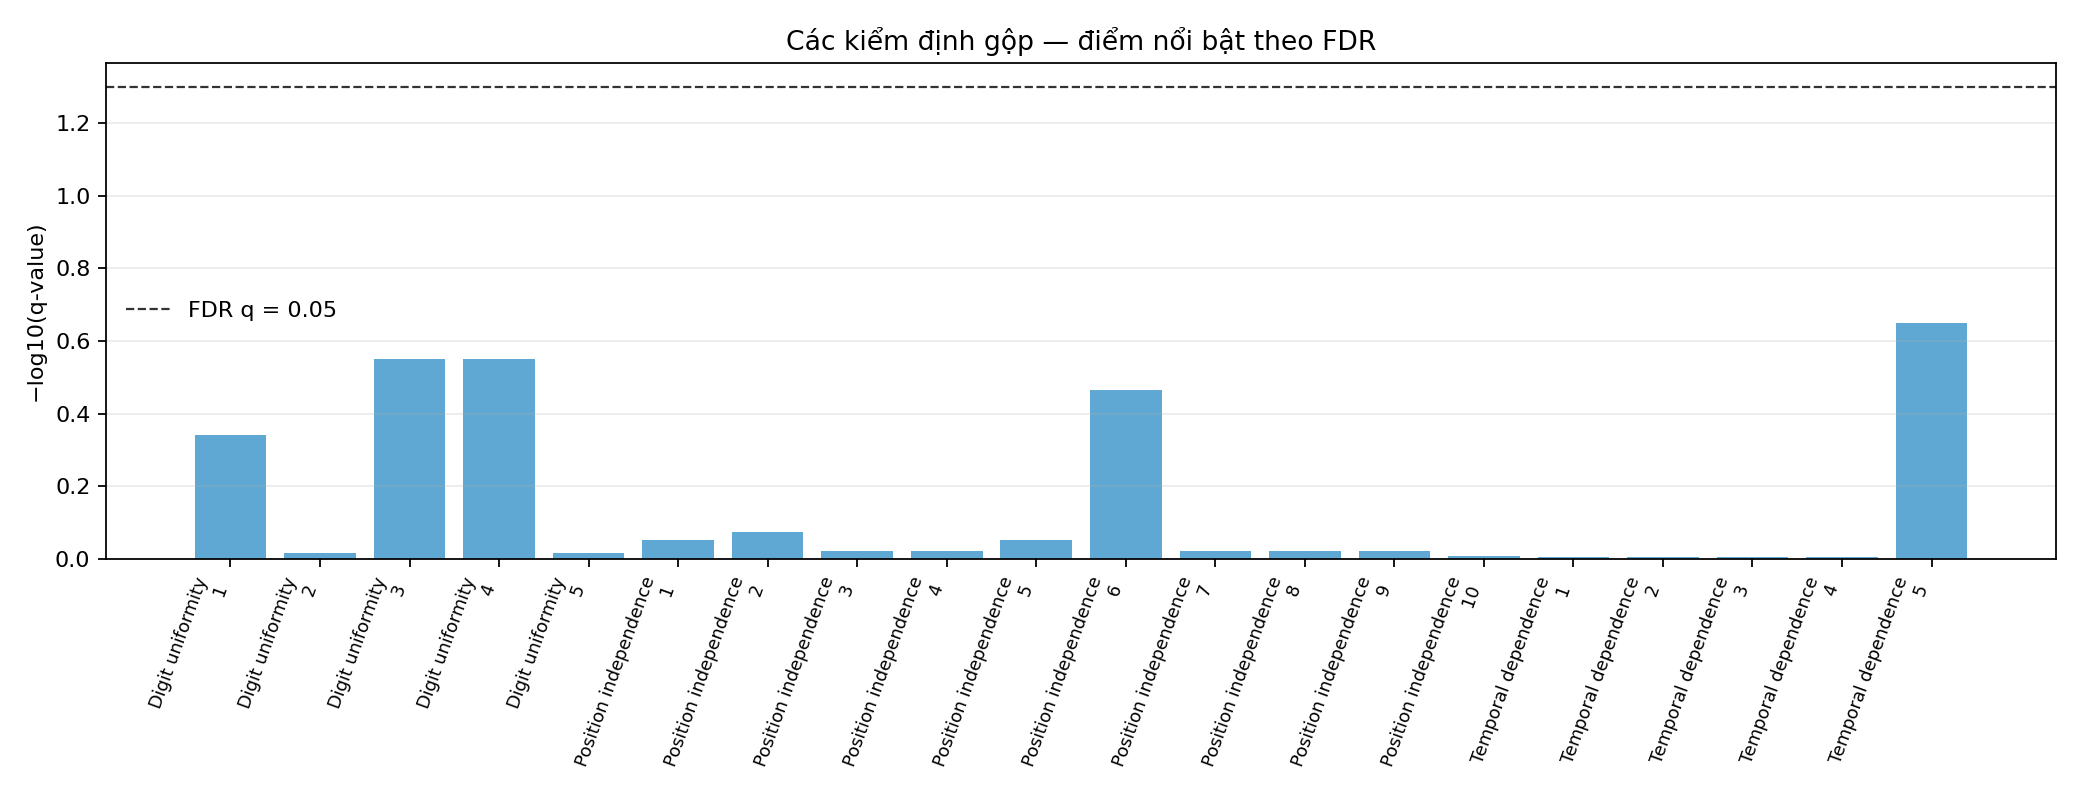
\includegraphics[width=0.92\linewidth]{../artifacts/p1_statistical_tests/04b_temporal_stability/figures/04_pooled_test_significance.png}\caption{Kết quả kiểm định gộp trong phân tích ổn định theo thời gian.}\label{fig:p1-significance}\end{figure}
\begin{figure}[H]\centering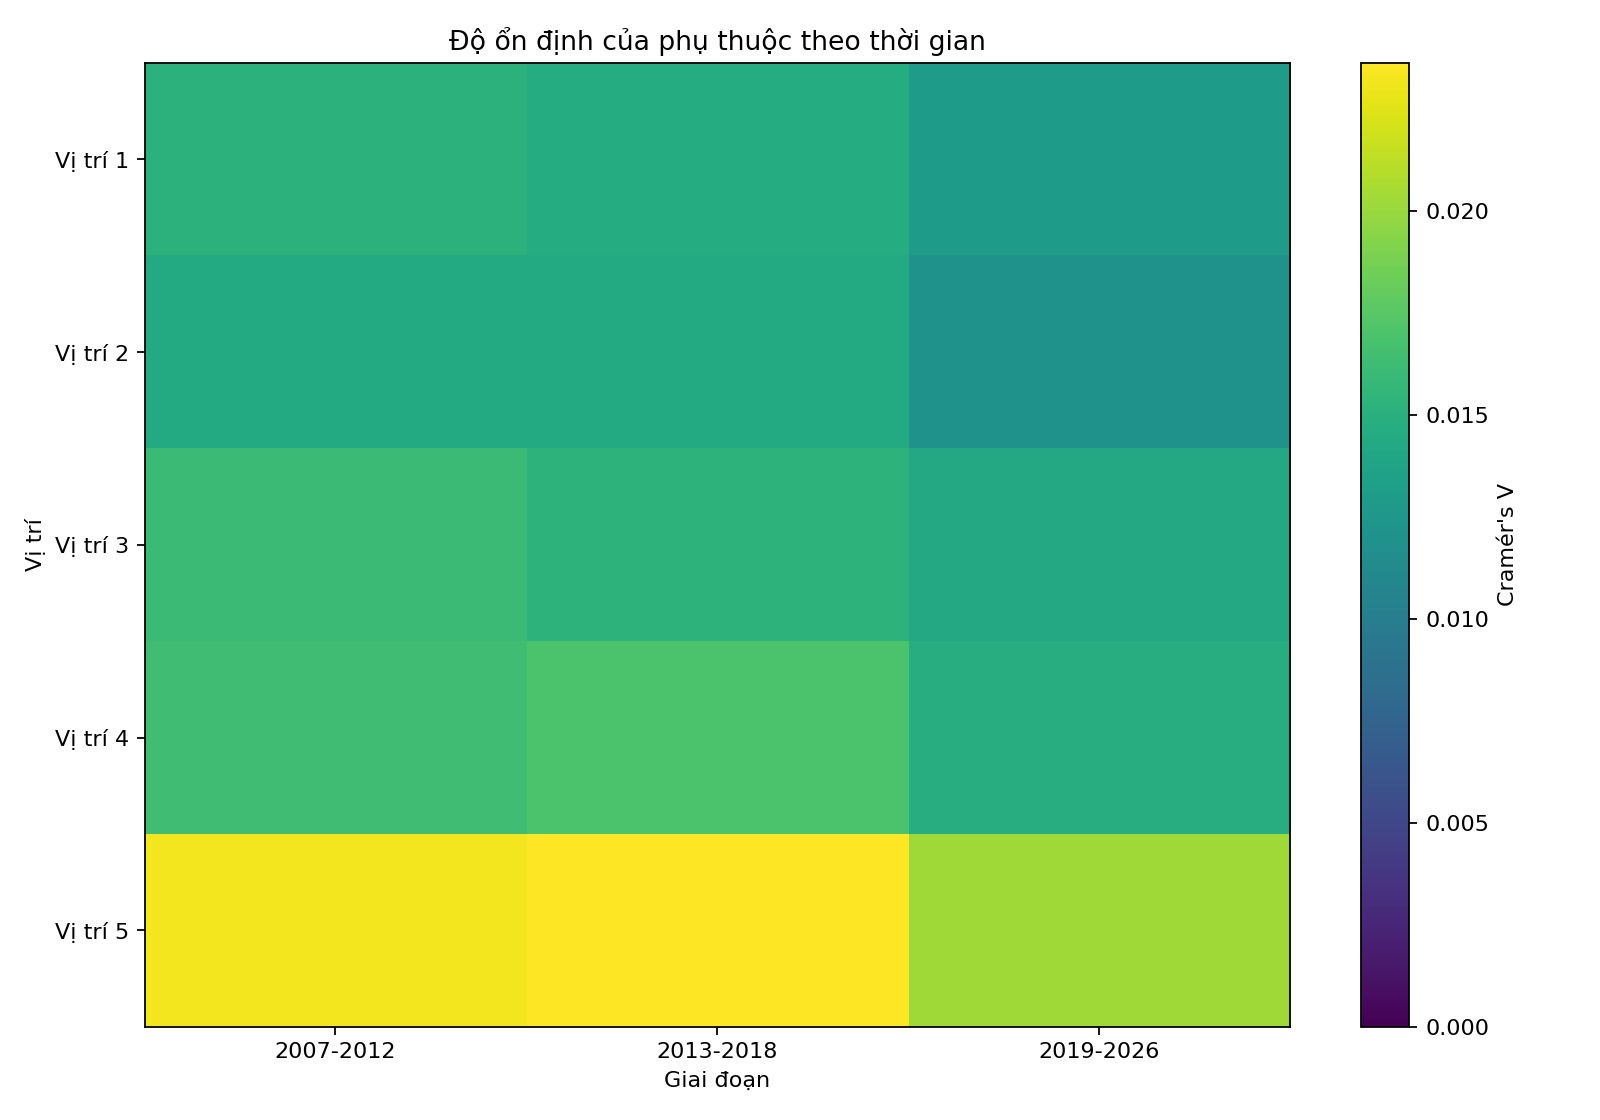
\includegraphics[width=0.92\linewidth]{../artifacts/p1_statistical_tests/04b_temporal_stability/figures/05_temporal_stability.png}\caption{Độ ổn định của các thống kê theo giai đoạn.}\label{fig:p1-stability}\end{figure}
\begin{figure}[H]\centering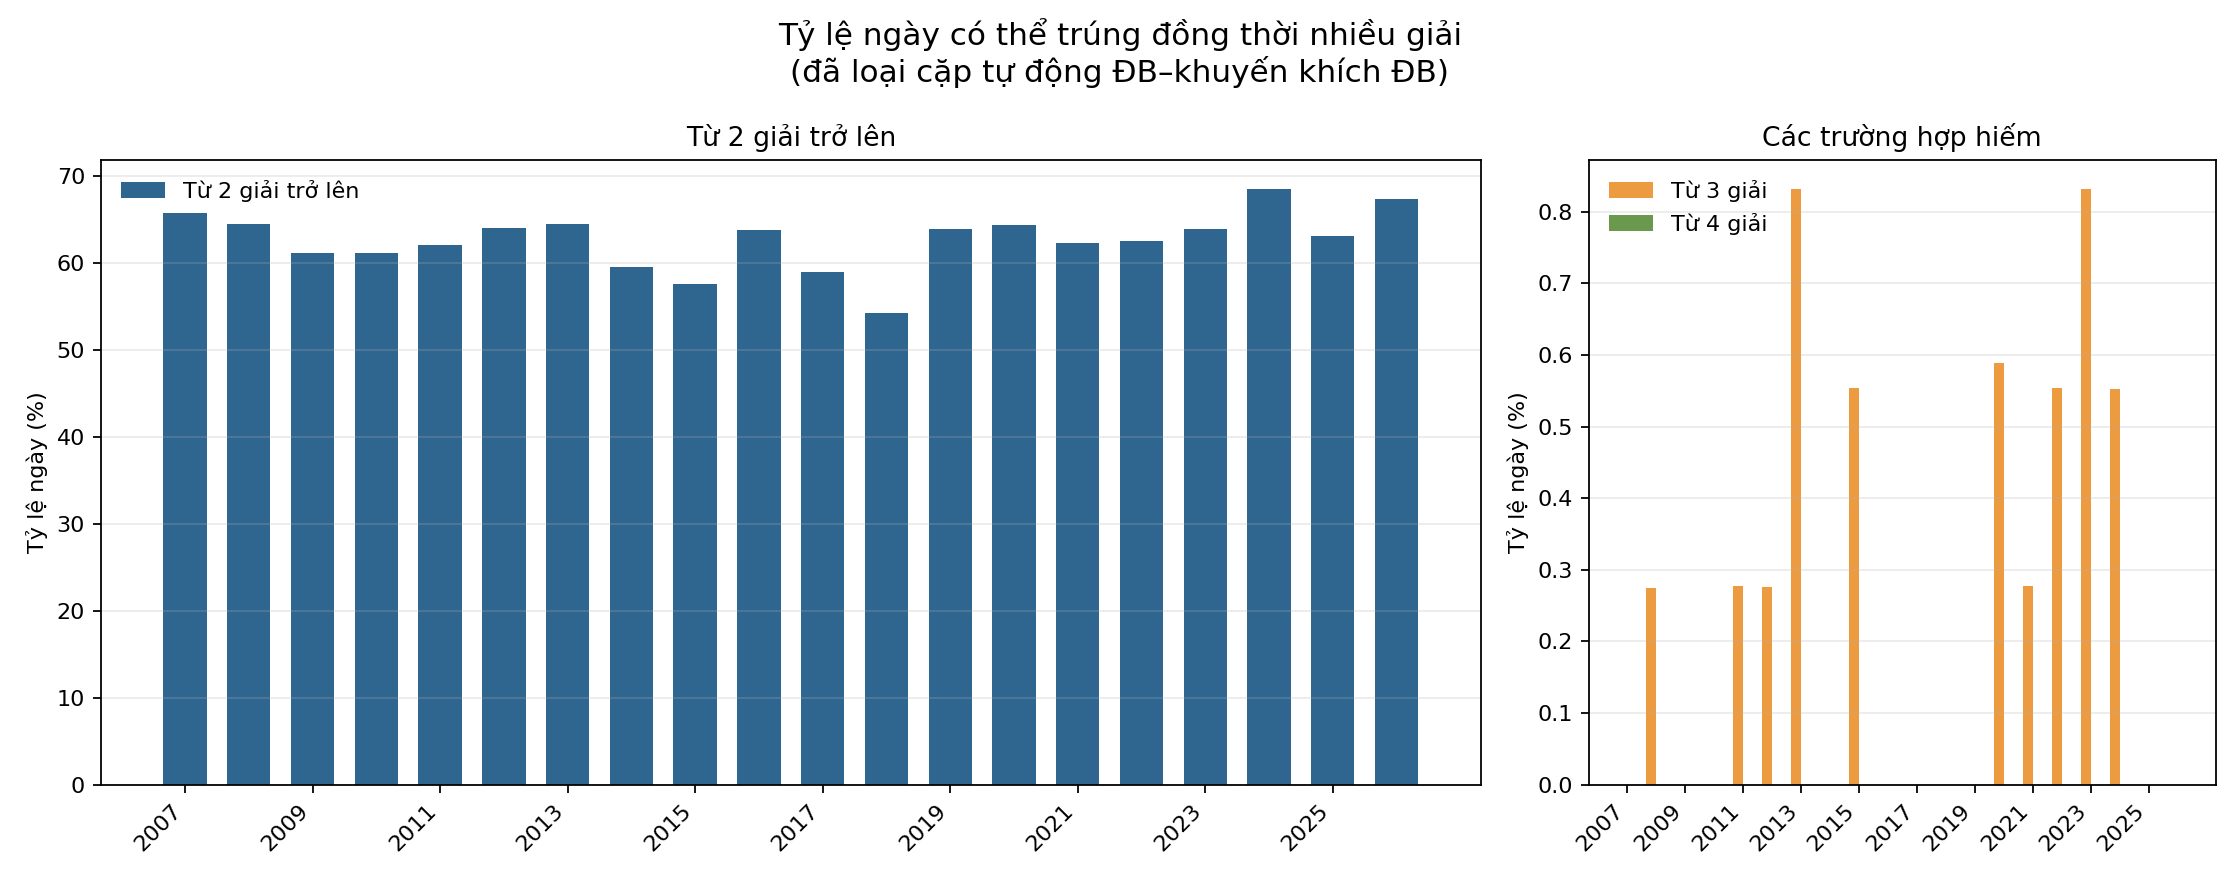
\includegraphics[width=0.92\linewidth]{../artifacts/p1_statistical_tests/04_temporal_randomness/figures/03_multi_win_rates_by_year.png}\caption{Tỷ lệ trúng đồng thời nhiều giải theo năm.}\label{fig:p1-multi}\end{figure}

\section{Kết luận P1}
Các kiểm định cung cấp bằng chứng nhất quán với một quá trình gần ngẫu nhiên ở mức độ cần thiết cho dự báo thực hành. Một vài sai lệch cục bộ có thể xuất hiện do kích thước mẫu lớn, do cơ chế nhiều giải trong cùng ngày hoặc do biến thiên ngẫu nhiên. Vì vậy, P1 chỉ cho phép chuyển sang kiểm tra dự báo ngoài mẫu; không cho phép khẳng định có lợi thế chơi.
